\section{Documentación EBX}

Para conocer las herramientas y funciones de EBX, este cuanta con su propia documentación en la cual se detalla desde el proceso de instalación hasta el manejo de cada uno de sus componentes.

Cabe mencionar que dicho manual puede obtenerse desde EBX haciendo clic en el botón de ayuda “?” ubicado en la parte superior derecha.

\begin{figure}[H]
    \centering
    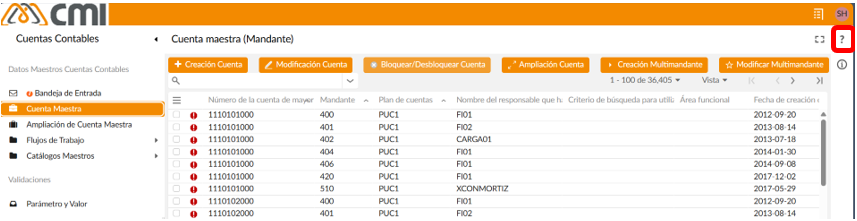
\includegraphics[width=0.8\textwidth]{DocumentacionEBX/ImgDocumentacion/DE01.png}
    \caption{Acceso a documentación a través del símbolo de “?”.}
\end{figure}

O bien dando clic en nuestro usuario, al desplegarse las opciones se encuentra el apartado de “Ayuda”.

\begin{figure}[H]
    \centering
    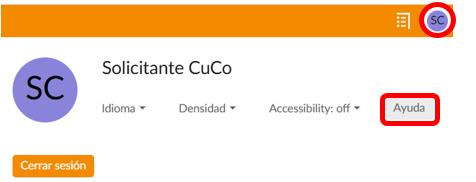
\includegraphics[width=0.8\textwidth]{DocumentacionEBX/ImgDocumentacion/DE02.png}
    \caption{Acceso a documentación a través del botón de ayuda.}
\end{figure}
